\documentclass{beamer}
\usepackage{amsfonts,amsmath,oldgerm}
\usepackage{graphicx}
\usetheme{sintef}

\newcommand{\testcolor}[1]{\colorbox{#1}{\textcolor{#1}{test}}~\texttt{#1}}

\usefonttheme[onlymath]{serif}

% Assicurati di avere un'immagine in assets/background o commenta la riga seguente
\titlebackground*{assets/background}

\newcommand{\hrefcol}[2]{\textcolor{cyan}{\href{#1}{#2}}}

\title{Parallel Image Stitching}
\subtitle{Performance Analysis of Concurrent Architectures in Python}
\author{\href{mailto:davide.lombardi2@edu.unifi.it}{Davide Lombardi}}
\date{July 20, 2026}

\begin{document}
\maketitle

% ============================================================
% SLIDE 1: Introduction
% ============================================================
\begin{frame}{Introduction}
  \begin{itemize}
    \item \textbf{Image Stitching:} combining multiple overlapping images into a single high-resolution panorama
    \item \textbf{Applications:} geospatial mapping, autonomous driving, virtual reality, consumer photography
    \item \textbf{The Problem:} the standard sequential pipeline scales poorly as resolution and dataset size grow
    \item \textbf{Objective:} evaluate Python concurrency paradigms against two language-specific bottlenecks:
      \begin{itemize}
        \item The \textbf{Global Interpreter Lock (GIL)} restricts true multi-threaded execution
        \item \textbf{Inter-Process Communication (IPC)} introduces serialization overhead
      \end{itemize}
  \end{itemize}
\end{frame}

% ============================================================
% SLIDE 2: Visual Overview (images + bullets)
% ============================================================
\begin{frame}{Visual Overview}
  \begin{columns}
    \begin{column}{0.55\textwidth}
      \begin{figure}[h]
          \centering
          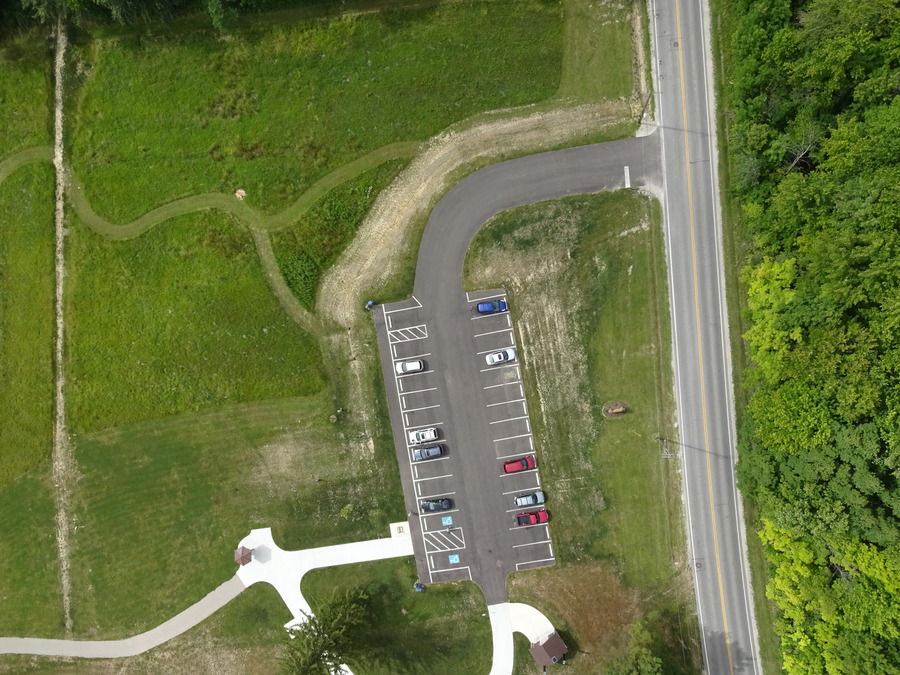
\includegraphics[width=0.48\textwidth,height=2.1cm,keepaspectratio]{img/0000.jpg}\hfill
          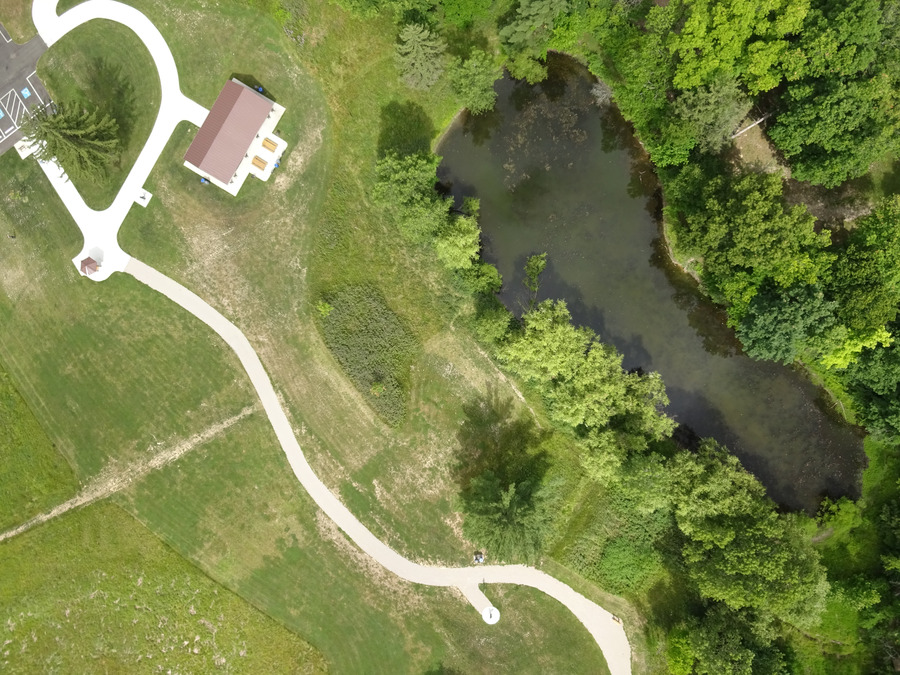
\includegraphics[width=0.48\textwidth,height=2.1cm,keepaspectratio]{img/0001.jpg}\\[0.15cm]
          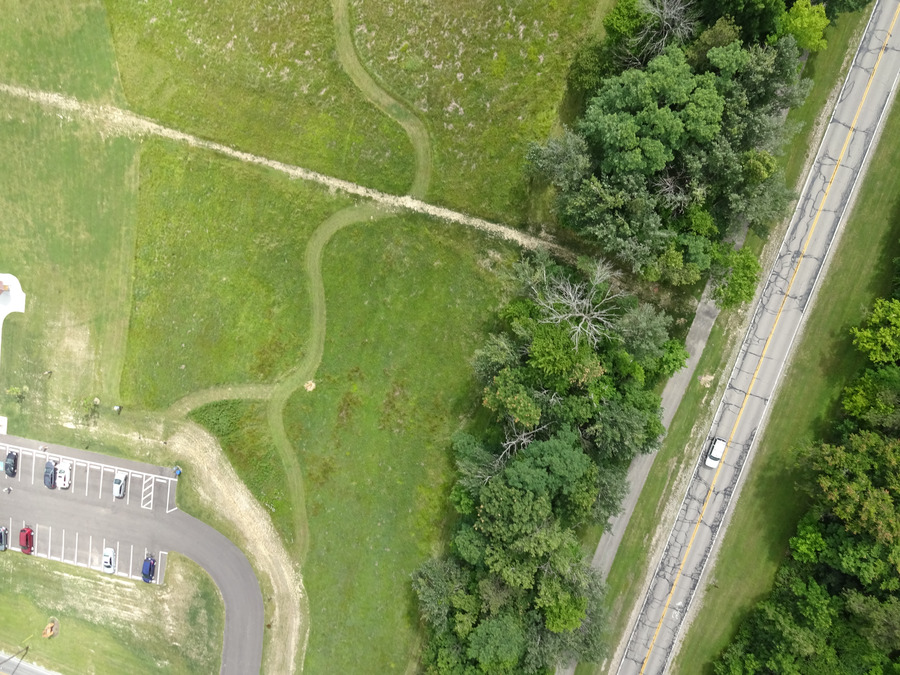
\includegraphics[width=0.48\textwidth,height=2.1cm,keepaspectratio]{img/0002.jpg}\hfill
          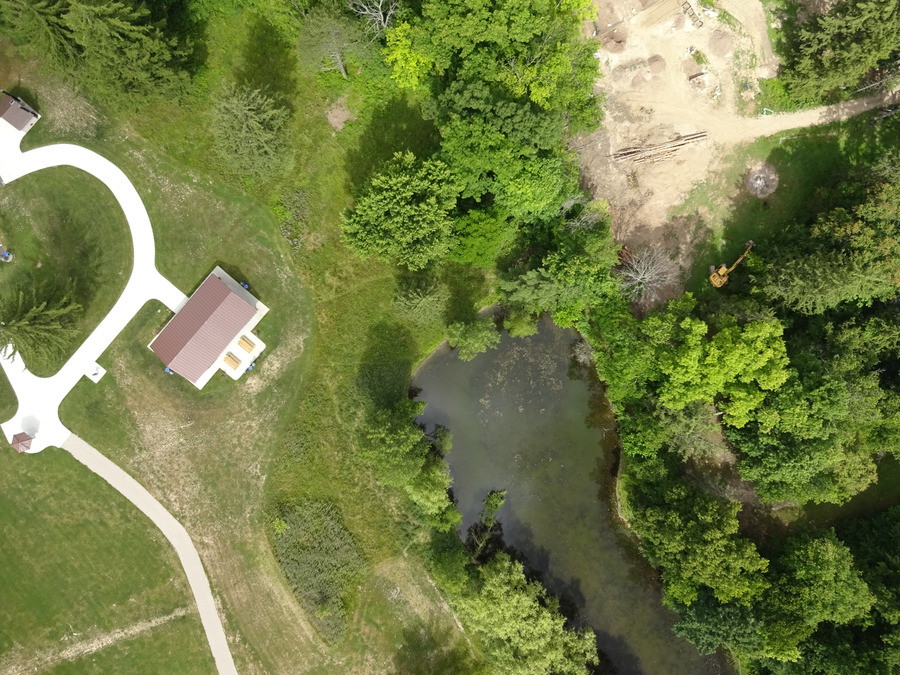
\includegraphics[width=0.48\textwidth,height=2.1cm,keepaspectratio]{img/0003.jpg}\\[0.3cm]
          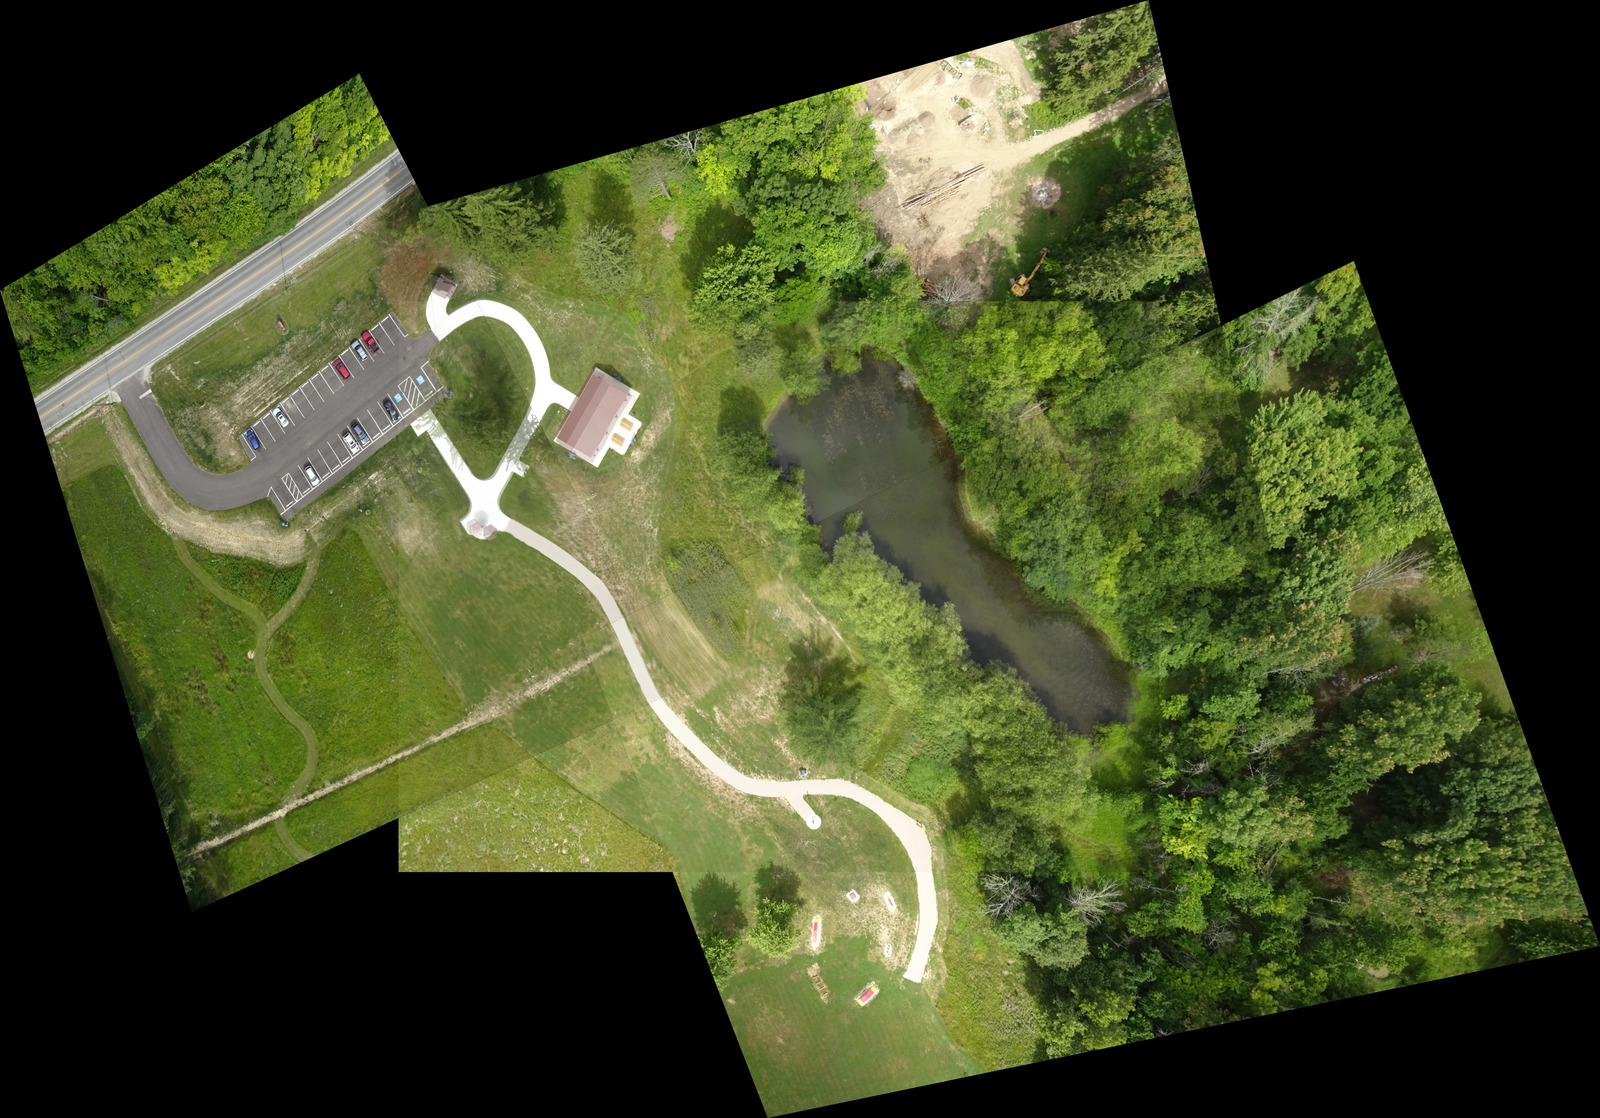
\includegraphics[width=\textwidth,height=2.6cm,keepaspectratio]{img/panorama_window_0_to_3.jpg}
          \caption{4 overlapping aerial frames merged into a unified panorama}
      \end{figure}
    \end{column}
    \begin{column}{0.45\textwidth}
      \begin{itemize}
        \item \textbf{Dataset:} OpenDroneMap aerial imagery, downsampled to 50\% resolution
        \item \textbf{Sliding window:} panoramas built from non-overlapping windows of 4 images at a time
        \item \textbf{Six architectures} benchmarked on this exact pipeline against a sequential baseline
      \end{itemize}
    \end{column}
  \end{columns}
\end{frame}

% ============================================================
% SLIDE 3: The Stitching Pipeline (1/2) — Feature Processing
% ============================================================
\begin{frame}{The Stitching Pipeline: Feature Processing}
  \begin{enumerate}
    \item \textbf{Feature Extraction (SIFT):}
      \begin{itemize}
        \item Detects scale-space extrema via the Difference of Gaussians
        \item Runs independently per image, so it is embarrassingly parallel
      \end{itemize}
    \item \textbf{Feature Matching (FLANN):}
      \begin{itemize}
        \item Compares 128-dimensional descriptors between adjacent frames
        \item Lowe's ratio test with $\tau < 0.7$ filters out spurious matches
      \end{itemize}
    \item \textbf{Homography Estimation (RANSAC):}
      \begin{itemize}
        \item Iteratively fits a $3\times3$ matrix $H$ that separates inliers from outliers
        \item Runtime is non-deterministic and depends on match quality
      \end{itemize}
  \end{enumerate}
\end{frame}

% ============================================================
% SLIDE 4: The Stitching Pipeline (2/2) — Merging & Bottlenecks
% ============================================================
\begin{frame}{The Stitching Pipeline: Merging \& the Structural Bottleneck}
  \begin{columns}
    \begin{column}{0.5\textwidth}
      \begin{block}{Warping \& Blending}
        \begin{itemize}
          \item Linear alpha blending removes visible seams between frames
          \item Heavy, vectorizable array manipulation
        \end{itemize}
      \end{block}
    \end{column}
    \begin{column}{0.5\textwidth}
      \begin{colorblock}[white]{sintefred}{Feature Re-extraction}
        \begin{itemize}
          \item Must run again on the updated canvas after every merge
          \item Canvas area grows monotonically: $A_n \approx A_0 + \sum_{i=1}^n \Delta A_i$
          \item \textbf{Strict dependency:} stitch $i$ cannot start until stitch $i-1$ is committed
        \end{itemize}
      \end{colorblock}
    \end{column}
  \end{columns}
  \vspace{0.3cm}
  This rigid, monotonically-growing sequential chain is the central obstacle every parallel architecture in this work has to work around
\end{frame}

% ============================================================
% SLIDE 5: Targeted Parallel Pipeline
% ============================================================
\begin{frame}{Targeted Parallel Pipeline}
  Addresses each bottleneck according to its computational nature. %\footnotesize{Hardware: 4 physical cores, 8 logical threads.}
  \normalsize
  \begin{itemize}
    \item \textbf{Threaded I/O:} image loading uses a \texttt{ThreadPoolExecutor}, since file reads release the GIL
    \item \textbf{Process-pool SIFT:} CPU-bound extraction uses independent processes to fully bypass the GIL
      \begin{itemize}
        \item Requires a pickling workaround. C++ \texttt{cv2.KeyPoint} objects are decomposed into plain tuples before crossing the process boundary
      \end{itemize}
    \item \textbf{Tiled Blending:} the output canvas is split into horizontal tiles blended concurrently
      \begin{itemize}
        \item NumPy array arithmetic releases the GIL, so threads are highly efficient here too
      \end{itemize}
  \end{itemize}
\end{frame}

% ============================================================
% SLIDE 6: Producer-Consumer Paradigm
% ============================================================
\begin{frame}{Producer-Consumer Paradigm}
  Decouples the independent extraction work from the sequential fold:
  \begin{itemize}
    \item \textbf{Temporal overlap:} SIFT extraction for image $i+1$ runs concurrently with the fold of image $i$
    \item \textbf{Architecture:} a producer thread dispatches every image to a warm process pool and pushes results onto a bounded \texttt{queue.Queue}, strictly in order
    \item \textbf{Zero-copy handoff:} producer and consumer share the same process address space, so passing an item costs only an object reference
    \item \textbf{Backpressure:} a fixed queue depth blocks the producer if it runs ahead of the consumer. This caps memory usage
  \end{itemize}
\end{frame}

% ============================================================
% SLIDE 7: MapReduce Paradigm
% ============================================================
\begin{frame}{MapReduce Paradigm}
  Restructures the fold into a binary merge tree:
  \begin{itemize}
    \item \textbf{Map phase:} SIFT extraction for all $n$ images runs concurrently
    \item \textbf{Reduce phase:} adjacent pairs such as $(0,1)$ and $(2,3)$ are stitched concurrently. The process repeats over $\lceil \log_2 n \rceil$ levels instead of $n-1$ sequential steps
    \item \textbf{The trade-off:} pairs are fixed by index rather than verified spatial overlap. This yields the highest peak speedup, but the result becomes geometrically unstable when a fixed pairing does not actually overlap
  \end{itemize}
\end{frame}

% ============================================================
% SLIDE 8: IPC Optimization Strategies
% ============================================================
\begin{frame}{IPC Optimization Strategies}
  Pickling roughly 13.5\,MB image arrays across process boundaries is expensive
  \begin{itemize}
    \item \textbf{Joblib:} the \texttt{loky} backend keeps worker processes alive across calls and automatically memory-maps arrays larger than 1\,MB to disk instead of pickling them
    \item \textbf{Shared Memory:} images are copied once into a \texttt{multiprocessing.shared\_memory} block. Workers then reconstruct a NumPy view instead of receiving a pickled copy
      \begin{itemize}
        \item Only the outbound transfer is optimized. Results still return via the normal pickled channel
        %\item Not a true zero-copy read: each worker copies the shared array into local memory once connected, then releases the connection immediately, to avoid unsafe cleanup while a worker is still attached
      \end{itemize}
  \end{itemize}
\end{frame}

% ============================================================
% CHAPTER DIVIDER
% ============================================================
\begin{chapter}[assets/background]{maincolor}{Performance Results}
\end{chapter}

% ============================================================
% SLIDE 9: Results — The Amdahl Ceiling (MAIN RESULT)
% ============================================================
\begin{frame}{Results: The Amdahl Ceiling}
  \begin{figure}[h]
      \centering
      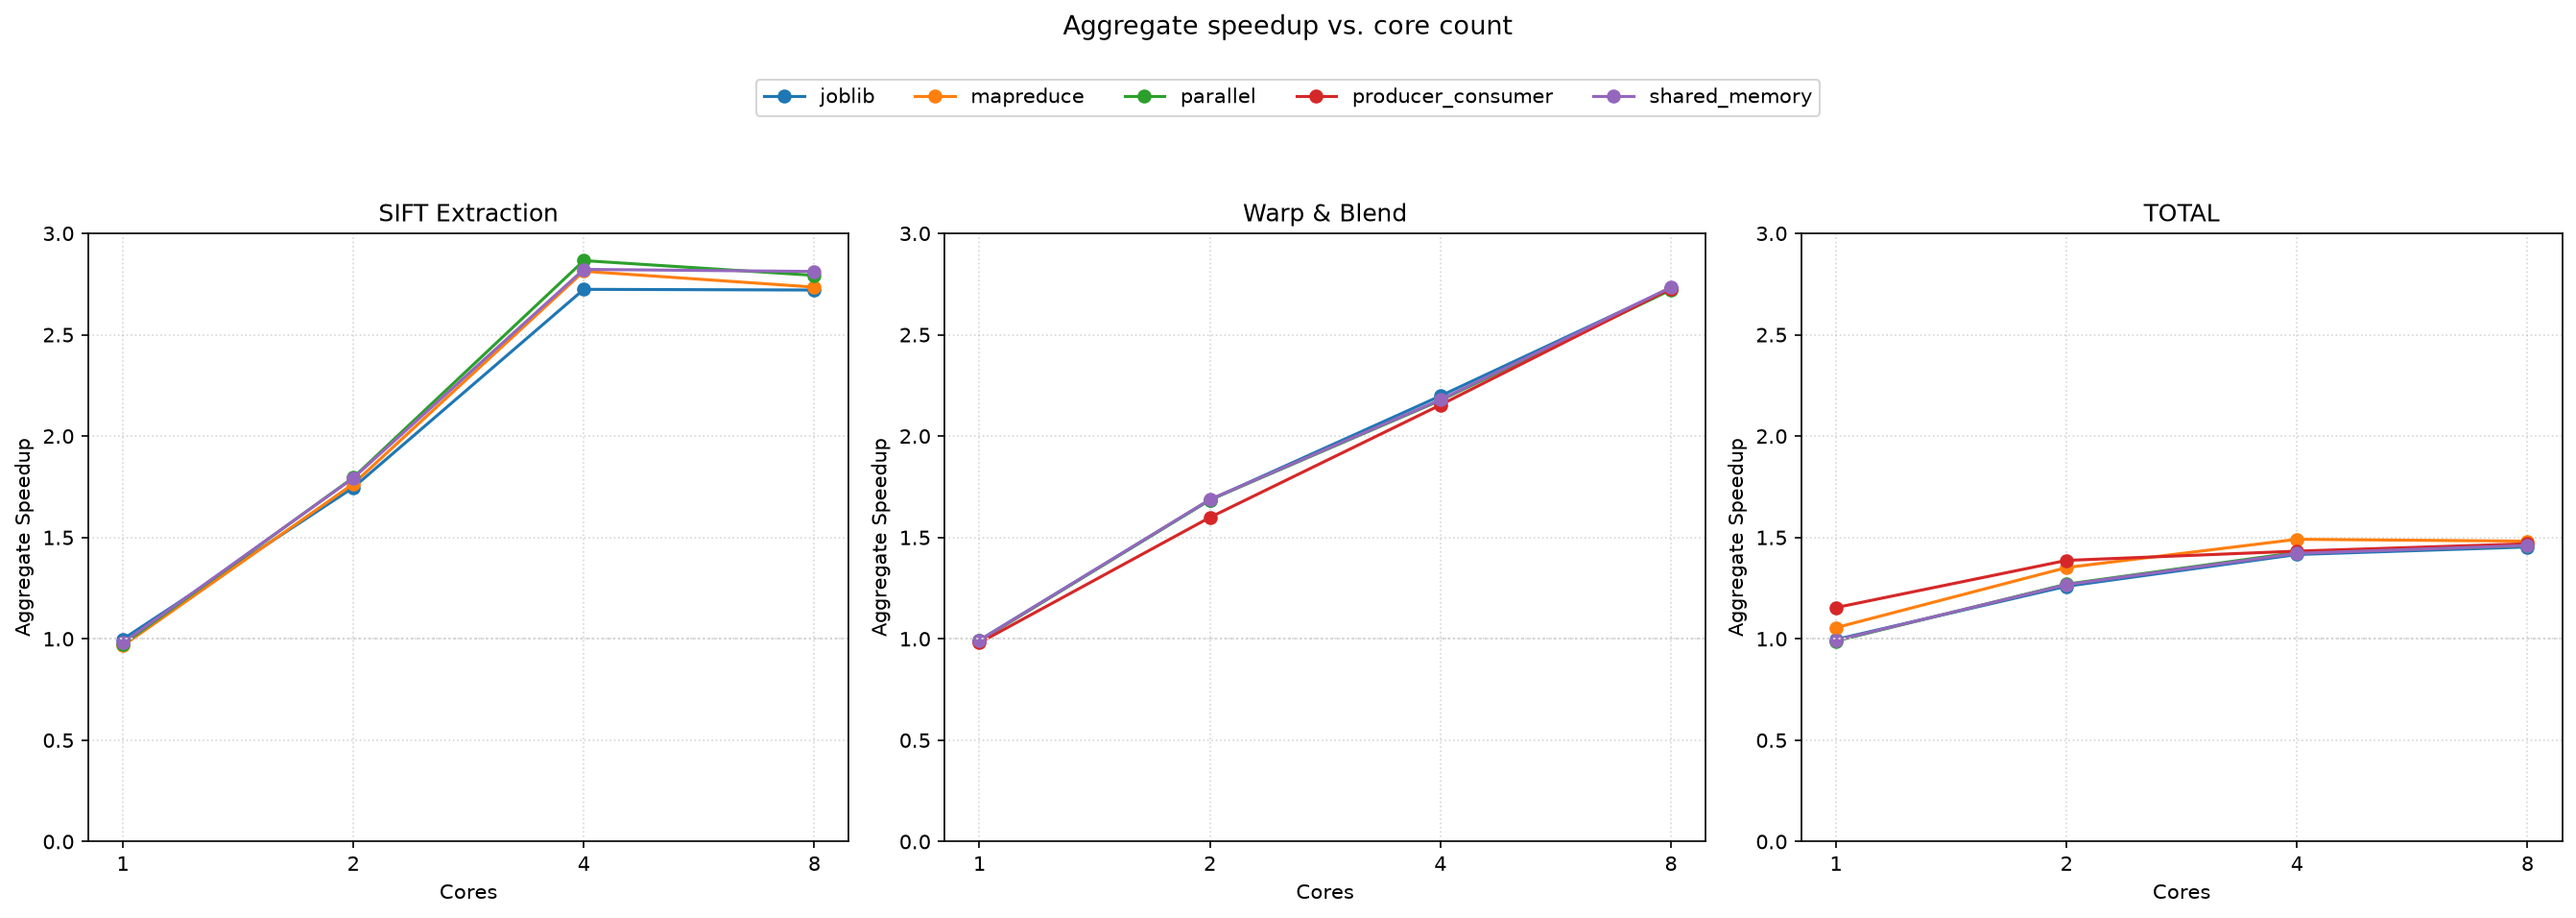
\includegraphics[width=0.95\textwidth]{img/speedup_vs_cores.png}
  \end{figure}
  \vspace{-0.1cm}
  \begin{itemize}
      \footnotesize
      \item \textbf{SIFT Extraction} plateaus at roughly 2.7--2.9$\times$ past 4 cores, due to task starvation with a small window
      \item \textbf{Warp \& Blend} scales almost linearly to 8 cores. This memory-bound work benefits from hyper-threading
      \item \textbf{TOTAL never exceeds roughly 1.5$\times$.} Feature re-extraction takes about 65\% of total time and stays fixed at approximately 14.5\,s: it is never parallelized by any architecture
  \end{itemize}
\end{frame}

% ============================================================
% SLIDE 10: Results — Stability & the MapReduce Trade-off
% ============================================================
\begin{frame}{Results: Stability \& the MapReduce Trade-off}
  \begin{figure}[h]
      \centering
      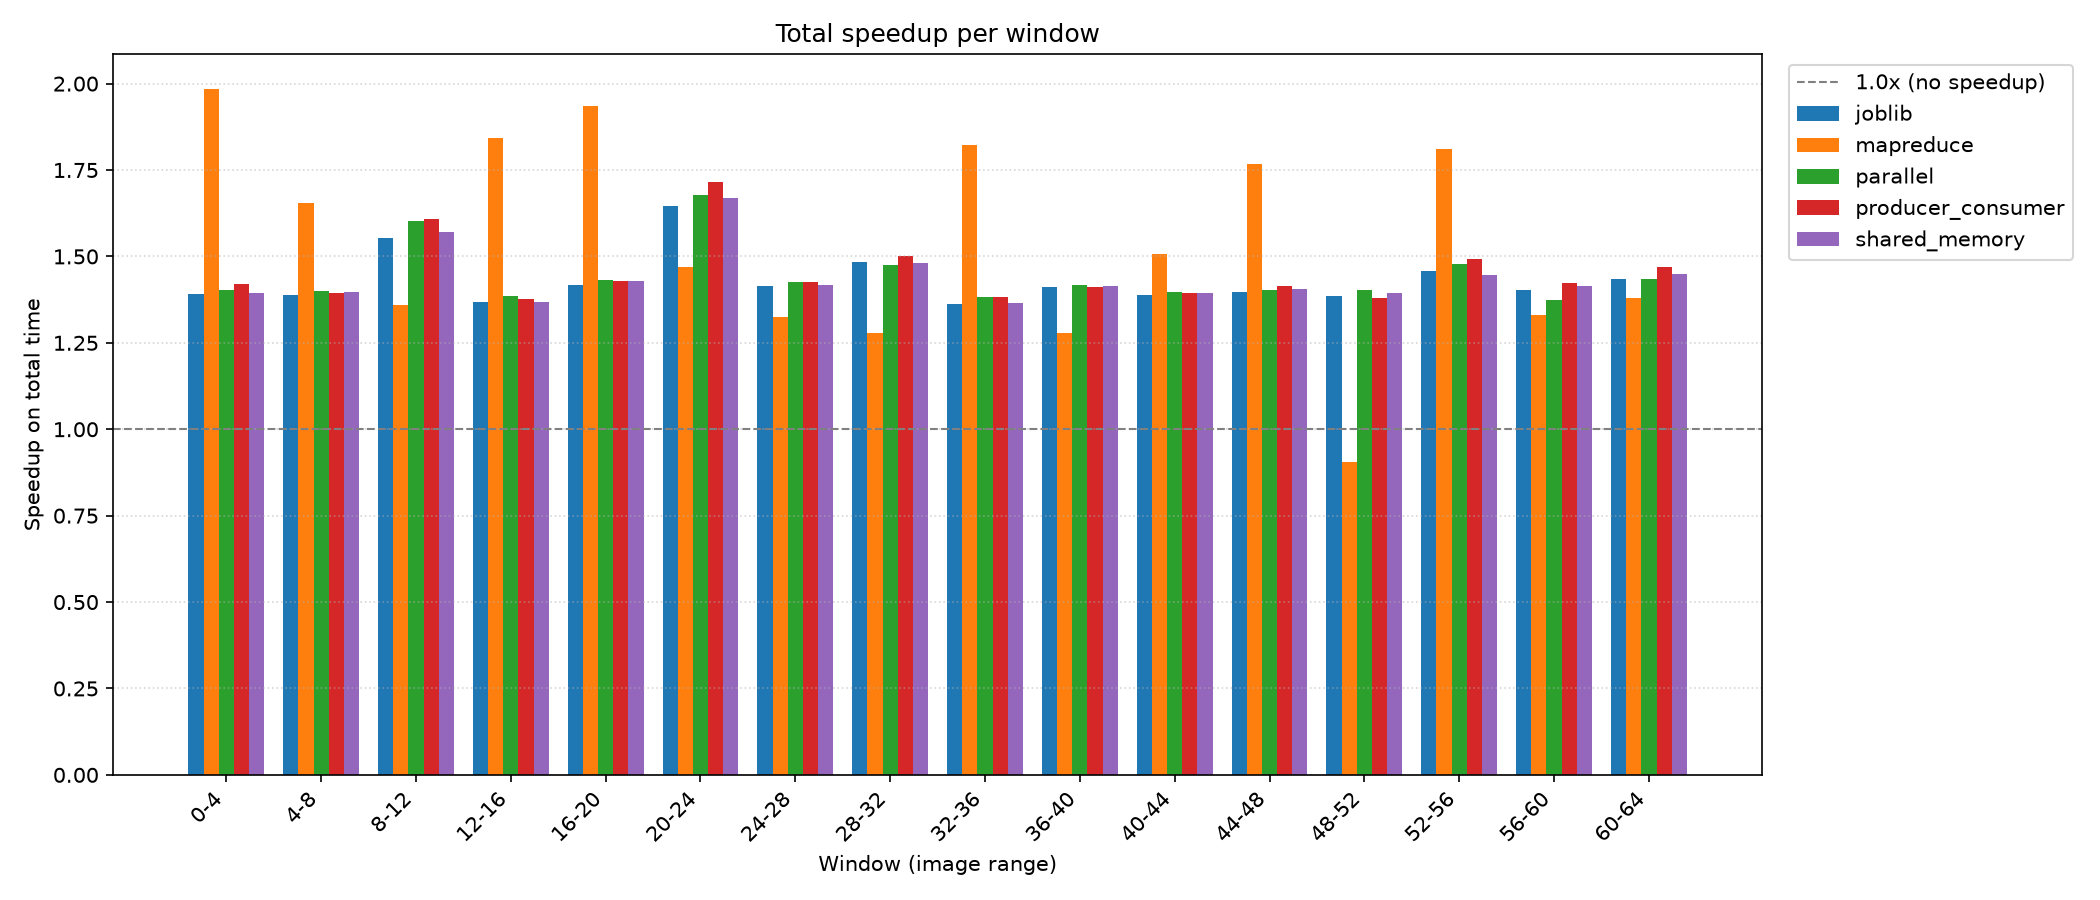
\includegraphics[width=0.80\textwidth]{img/speedup_total_per_window_4c_4s.png}
  \end{figure}
  \vspace{-0.1cm}
  \begin{itemize}
      \footnotesize
      \item \textbf{Linear-fold pipelines} are highly stable at 1.3$\times$ to 1.7$\times$ on every window
      \item \textbf{MapReduce} peaks near 2.0$\times$ but drops to 0.91$\times$
      \item \textbf{Why:} tree pairing is fixed by index rather than verified spatial overlap, so a geometrically unlucky pair has no fallback
  \end{itemize}
\end{frame}

% ============================================================
% SLIDE 11: Best Configuration / Key Numbers
% ============================================================
\begin{frame}{Key Numbers}
  \begin{columns}
    \begin{column}{0.48\textwidth}
      \begin{colorblock}[white]{sintefblu1}{Isolated Phases}
        \begin{itemize}
          \item SIFT Extraction peaks at \textbf{2.9$\times$} at 4 cores, then plateaus
          \item Warp \& Blend is still rising at 8 cores, reaching \textbf{2.7$\times$}
        \end{itemize}
      \end{colorblock}
    \end{column}
    \begin{column}{0.48\textwidth}
      \begin{colorblock}[white]{sintefred}{End-to-End}
        \begin{itemize}
          \item TOTAL speedup is capped at \textbf{roughly 1.5$\times$}
          \item MapReduce has the lowest average time, 21.1\,s, and the highest peak, 2.0$\times$, but is the least predictable
          \item The four IPC-optimized linear-fold variants differ by \textbf{under 1\%} from each other
        \end{itemize}
      \end{colorblock}
    \end{column}
  \end{columns}
\end{frame}

% ============================================================
% SLIDE 12: Conclusions
% ============================================================
\begin{frame}{Conclusions}
  \begin{itemize}
    \item Isolated CPU-bound and I/O-bound tasks overcome the GIL cleanly with targeted \texttt{multiprocessing} and \texttt{threading} %Matching each phase to the right paradigm matters more than the tool itself
    \item \textbf{IPC optimization gives diminishing returns} at this scale. Engineering effort on serialization, via Joblib and shared memory, yielded under 1\% gain over the simplest process-pool baseline
    \item \textbf{Main Lesson:} true end-to-end scalability needs functional decomposition, as in MapReduce's merge tree, rather than retrofitting concurrency onto a rigid sequence. This comes at the cost of predictability
    \item \textbf{Future Work:} algorithmic restructuring of the re-extraction phase or offloading the sequential chain to GPUs
  \end{itemize}
\end{frame}

\backmatter

% ============================================================
% BACKUP SLIDE (for Q&A only — not part of the timed talk)
% ============================================================
\begin{frame}{Per-Phase Speedup as Cores Increase}
  \begin{columns}
    \begin{column}{0.5\textwidth}
      \begin{figure}
          \centering
          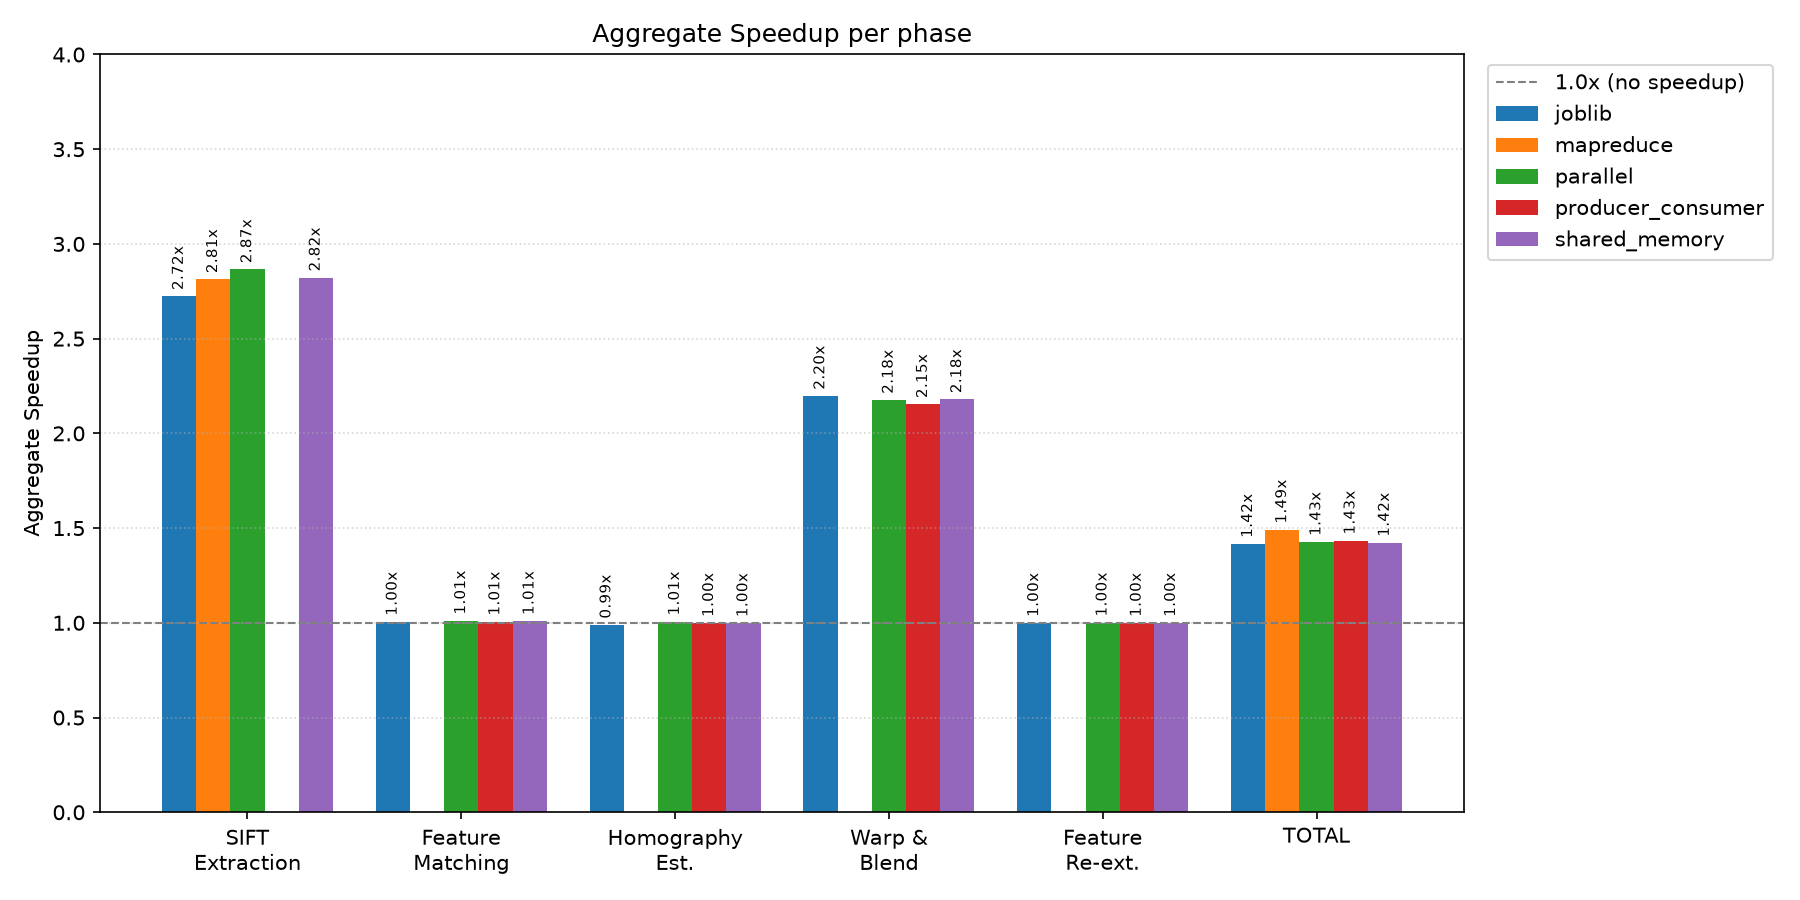
\includegraphics[width=0.95\textwidth]{img/perphase_4core.png}
          \caption{4 cores}
      \end{figure}
    \end{column}
    \begin{column}{0.5\textwidth}
      \begin{figure}
          \centering
          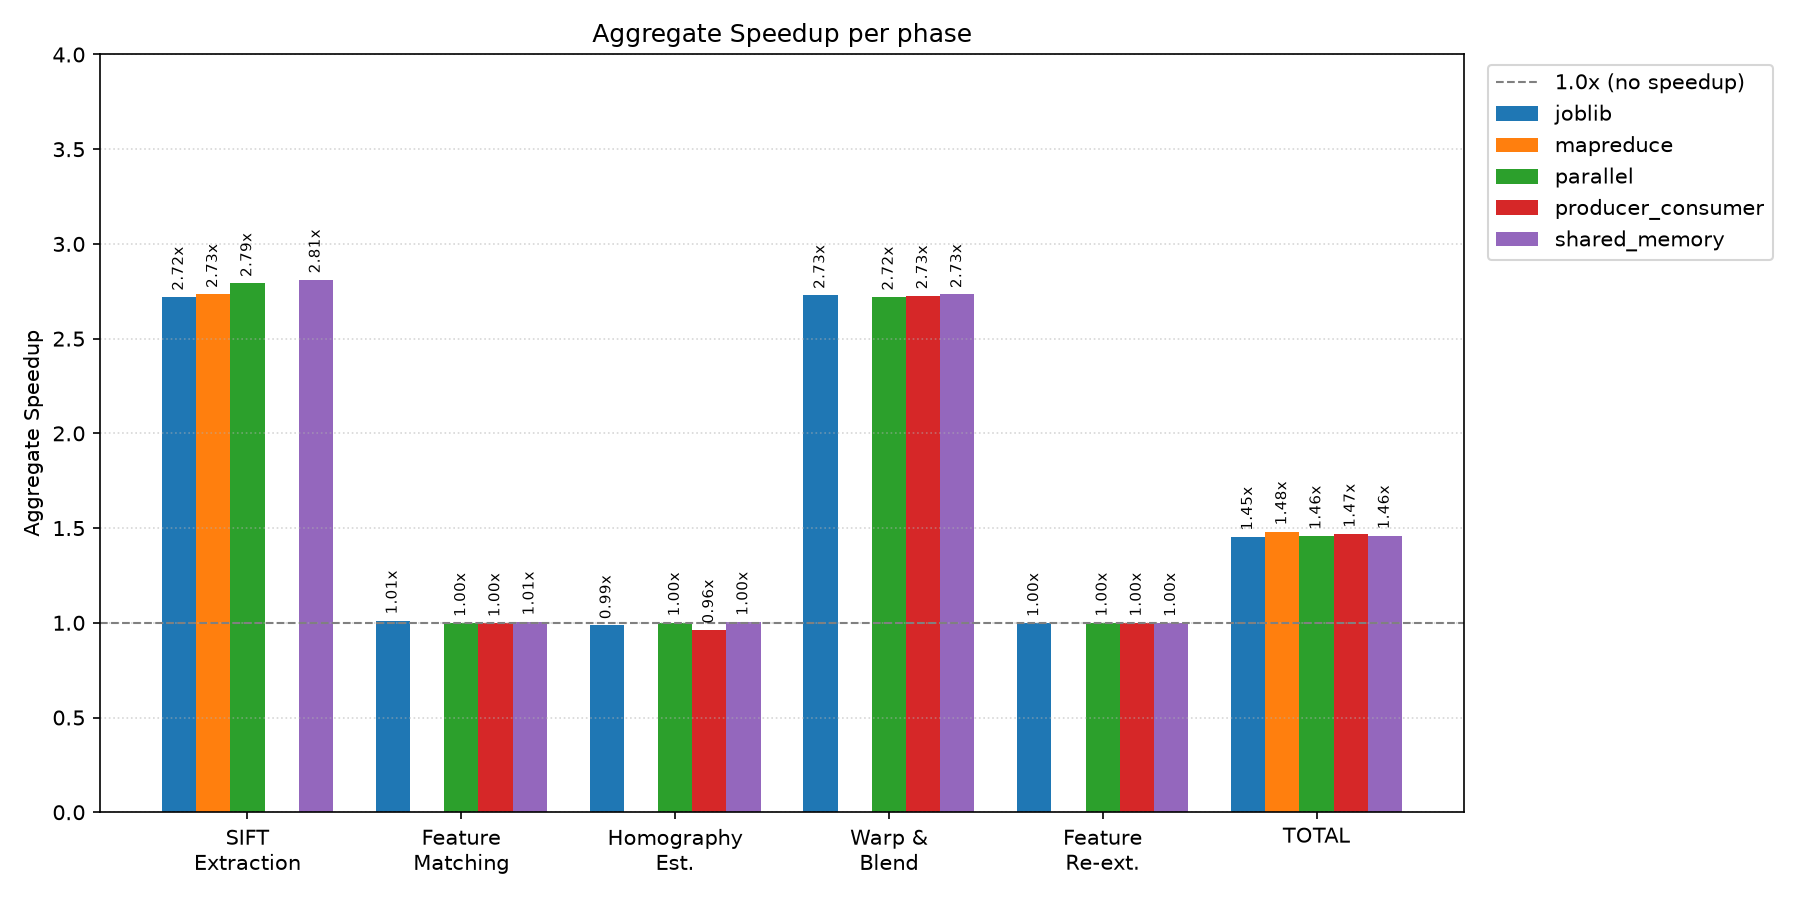
\includegraphics[width=0.95\textwidth]{img/perphase_8core.png}
          \caption{8 cores}
      \end{figure}
    \end{column}
  \end{columns}
  \begin{itemize}
      \footnotesize
      \item Match, Homography and Re-extraction stay flat at about 1.0$\times$ at every core count. None of the six pipelines ever parallelizes them
      \item At 8 cores with window size 4, only 4 tasks feed an 8-worker pool. This looks like a hardware plateau, but is it?
  \end{itemize}
\end{frame}

% ============================================================
% BACKUP SLIDE 2 (for Q&A only — window size effect)
% ============================================================
\begin{frame}{Task Starvation, Not a Hardware Limit}
  \begin{columns}
    \begin{column}{0.5\textwidth}
      \begin{figure}
          \centering
          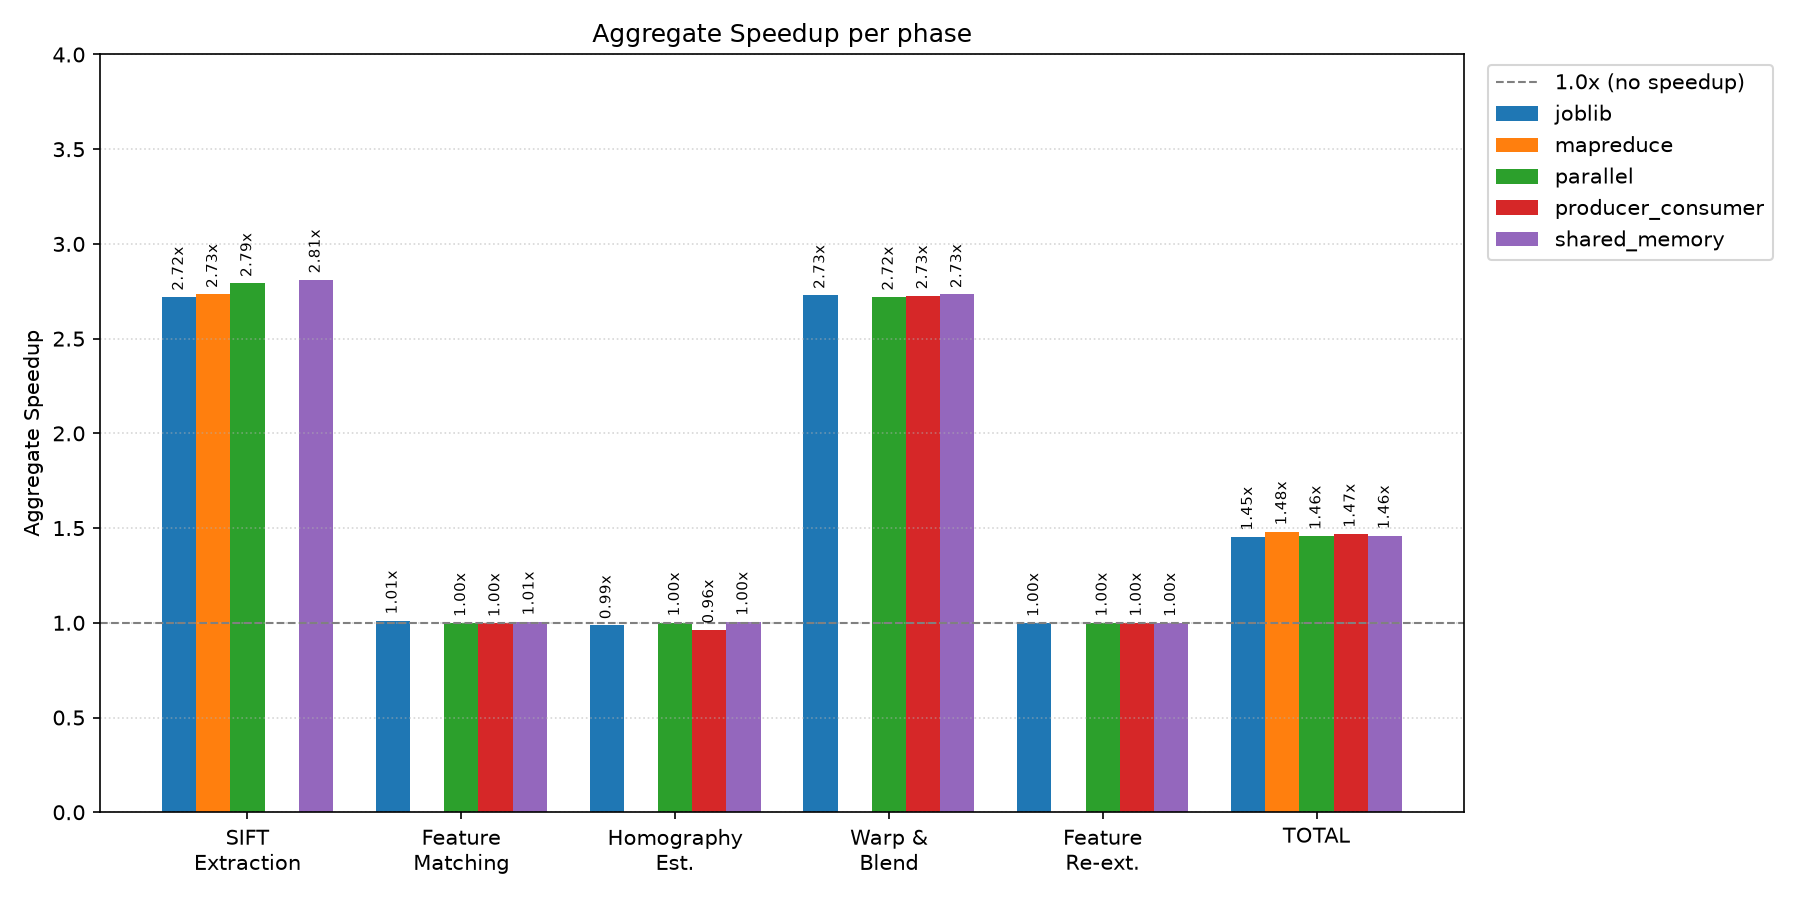
\includegraphics[width=0.95\textwidth]{img/perphase_8core.png}
          \caption{8 cores, window size 4}
      \end{figure}
    \end{column}
    \begin{column}{0.5\textwidth}
      \begin{figure}
          \centering
          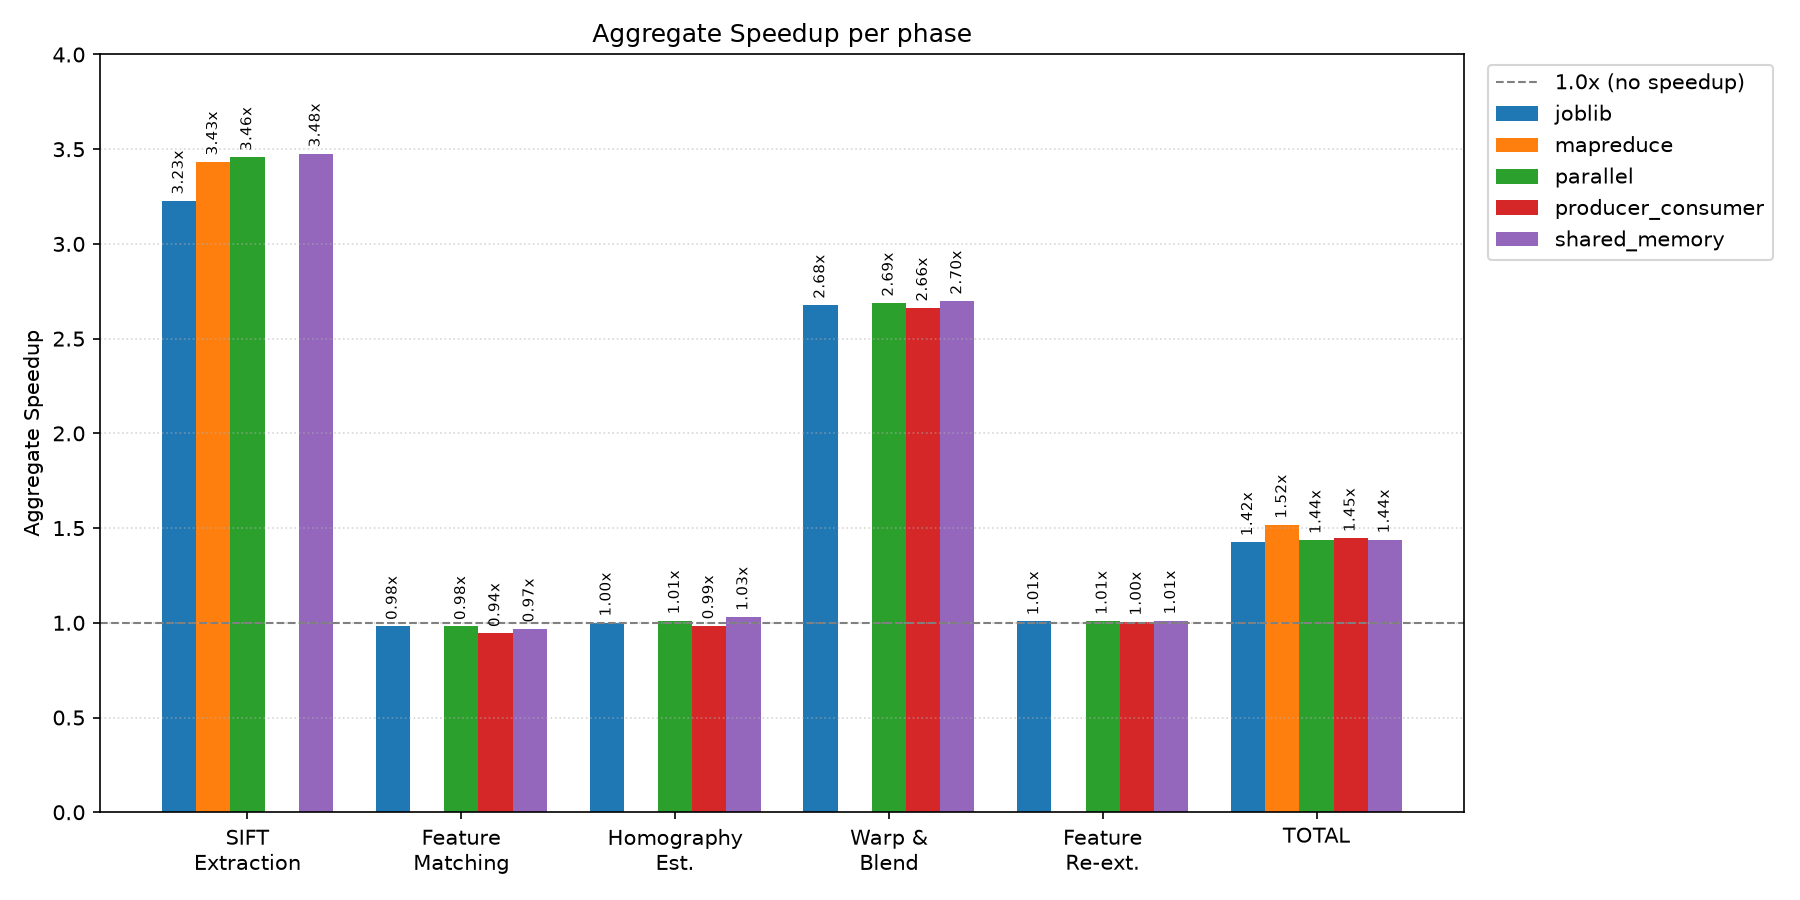
\includegraphics[width=0.95\textwidth]{img/perphase_8core_window8.png}
          \caption{8 cores, window size 8}
      \end{figure}
    \end{column}
  \end{columns}
  \begin{itemize}
      \footnotesize
      \item With window size 4, only 4 tasks feed an 8-worker pool. Half the pool sits idle, and dispatch overhead is disproportionate to the actual computation
      \item Doubling the window to 8 images fully populates the pool. SIFT Extraction breaks past the 2.7--2.8$\times$ plateau and reaches roughly 3.2--3.5$\times$
      \item \textbf{Confirms} that the earlier plateau was task starvation, not a hardware ceiling. Hyper-threading limits still apply, but only once the pool is actually full
  \end{itemize}
\end{frame}

\end{document}